\documentclass{article}
\usepackage{graphicx} % new way of doing eps files
\usepackage{listings} % nice code layout
\usepackage[usenames]{color} % color
\definecolor{listinggray}{gray}{0.9}
\definecolor{graphgray}{gray}{0.7}
\definecolor{ans}{rgb}{1,0,0}
\definecolor{blue}{rgb}{0,0,1}
% \Verilog{title}{label}{file}
\newcommand{\Verilog}[3]{
  \lstset{language=Verilog}
  \lstset{backgroundcolor=\color{listinggray},rulecolor=\color{blue}}
  \lstset{linewidth=\textwidth}
  \lstset{commentstyle=\textit, stringstyle=\upshape,showspaces=false}
  \lstset{frame=tb}
  \lstinputlisting[caption={#1},label={#2}]{#3}
}


\author{Josh Young}
\title{Lab 12}

\begin{document}
\maketitle

\section{Introduction}
In Lab 12, the user is required to test the pipeline that was created in lab 11 by creating their own instruction set and verifying the results. The pipeline consists of 5 stages, which are Fetch, Decode, Execute, Memory, and Write Back. With these 5 stages, the user was able to simulate a full MIPS machine to a degree, however there are limitations to the pipeline since it doesn't include a forwarding unit. This means that in order to ensure that no data hazards were developed, it was of paramount importance to place 4 no-ops between each actual instruction. That way, when the fetch stage gets an instruction, there will not be the possiblity of calling on a register that was used on the previous instruction. The pipeline was simulated using verilog code via Vivado and the instruction set was modified using Notepad.

\section{Interface}
As stated before, there are 5 stages to the MIPS machine pipeline. The instruction set and register file were modified in order to create a simple program to run on the pipeline. The instructions are 32 bit binary numbers (machine code) and are essentially just assembly commands. In this case, an add instruction was used to count by 17 and the result was stored and rewritten in register 9 after each iteration. Other than these files, the pipeline is self sufficient and doesn't require inputs from the user. 

\section{Design}
The pipeline begins with the Fetch stage. This consists of a multiplexer and an adder to come up with program counts in order to fetch instructions from memory. Once the instruction has been fetched, the signal reaches the second part of the pipeline, the Decode stage. Here, the instruction's bits are grouped and distributed across a sign extender, and register file to in order to get values from the registers. After that, the signals reach the Execute stage which encompasses more multiplexers, and an ALU. After the ALU calculates a result, the result as well as other signals reaches the next stage in the pipeline, the Memory stage. Here is were the system finds out where to branch, as well as read and write. After the Memory stage, the pipeline finally reaches the last stage which is the Writeback stage. This is were the last of the signals loop back to the fetch and decode stage.

\section{Implementation}
The code used for constructing the pipeline can be seen in Listing~\ref{code:pipeline} on page~\pageref{code:pipeline} and the instruction set that was ran can be seen in Figure~\ref{fig:one}.

\Verilog{Verilog code for constructing the pipeline.}{code:pipeline}{../code/pipeline.v}

\section{Test Bench Design}
The lab required implementation of a testbench for the pipeline, but in this case, everything was self contained so the testbench is the same as the pipeline code; however, the instruction set was modified.

\section{Simulation}
The timing diagram shows that the pipeline is able to augment the program count and run autonomously as well as run through the instructions and calculate the correct result based off of given instructions. The pipeline also stores the result in the proper register. The timing diagram for the pipeline can be viewed in Figure~\ref{fig:test}. 
\section{Conclusions}
The goal for Lab 12 was to further test the pipeline by creating a new instruction set and verify the results given by the pipeline. By viewing Figure 2, one can see that the pipeline was able to fetch, decode, and execute the instruction as well as go through the memory and write back stages, demonstrating that the pipeline is working in proper order.
\begin{figure}
	\begin{center}
		\caption{Simple Instruction Set.}\label{fig:one}
		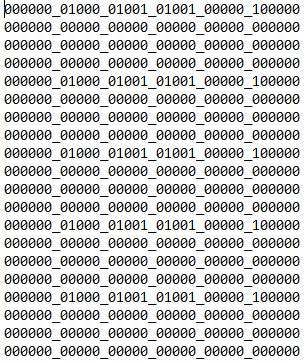
\includegraphics[width=0.9\textwidth]{../images/instructions.png}
	\end{center}
\end{figure}
\begin{figure}
	\begin{center}
		\caption{Timing diagram for the pipeline test.}\label{fig:test}
		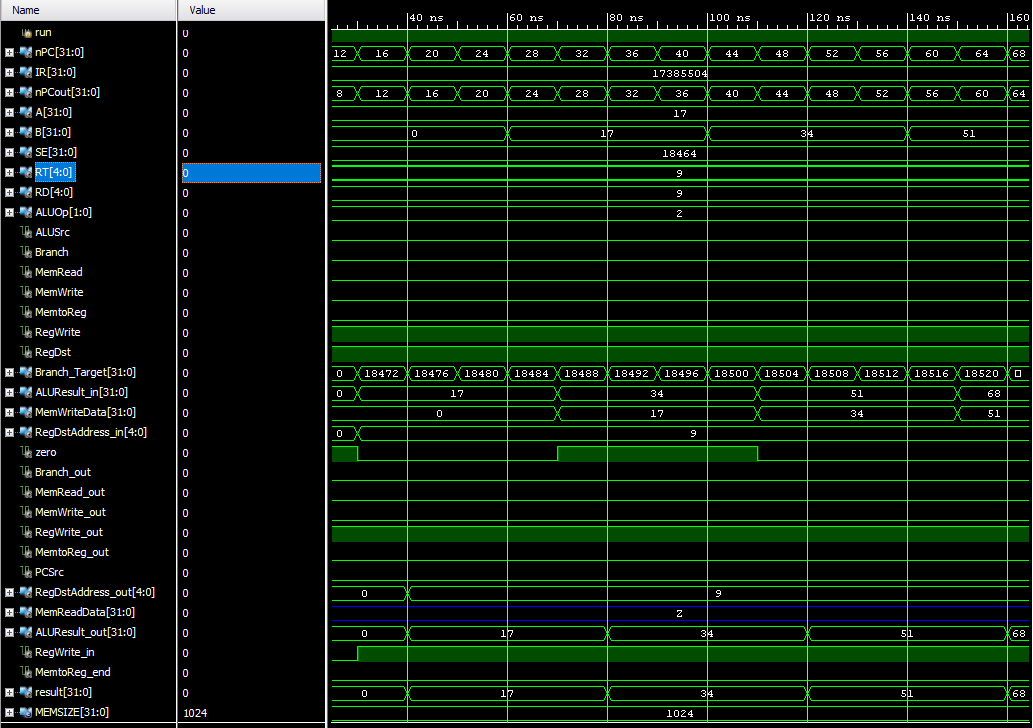
\includegraphics[width=0.9\textwidth]{../images/instructionstest.png}
	\end{center}
\end{figure}



\end{document} 